\documentclass[hyperref={pdfpagelabels=false}]{beamer}
\usepackage{pgfplots}
\usepackage[normalem]{ulem}
\usepackage{amsmath}
\usepackage{xcolor}
\usepackage{listings}

\pgfplotsset{width=10cm,compat=1.8}

\definecolor{darkblue}{RGB}{35,69,177}
\definecolor{darkred}{rgb}{0.6,0,0}

\newcommand\redout{\bgroup\markoverwith
{\textcolor{darkred}{\rule[.5ex]{2pt}{0.4pt}}}\ULon}

% \title{Hundert Leute haben wir gefragt: Wie l\"osen Sie R\"atsel in Curry?}   
% \author{Sandra Dylus} 
% \date{\today} 

\usetheme{Pittsburgh}
\setbeamertemplate{navigation symbols}{}
\begin{document}


\note{
Ich moechte heute die Ergebnisse einer kleinen
``Fallstudie'', die ich im kleinen Rahmen durchgef\"uhrt habe,
vorstellen -- wobei Ergebnisse vermutlich nicht der richtige Begriff
ist. %
Vielmehr moechte ich die Gelegenheit nutzen, meine Gedanken einmal
laut auszusprechen und meine Gedanke mit euch diskutieren. %
Letztendlich kommen hier ja doch sehr unterschiedliche Charaktere
bzgl. der Herangehensweise von Problemen zusammen.

Kurz zum Titel: da es sich hier um eine Anspielung auf eine Spiel-Show
aus den 90ern handelt, ist der Titel leider etwas unpr\"azise. %
Ich habe n\"amlich nur zehn Leute gefragt. %
}
\begin{frame}
\centering
\Large {\color{darkblue}$\stackrel{{\color{white}{\text{Zehn}}}}{\text{Hundert}}$ Leute haben wir gefragt: Wie l\"osen Sie R\"atsel
in Curry?}
\vfill
\normalsize
Sandra Dylus
\vfill
\today
\end{frame} 

\note{
Des Weiteren habe ich die Formulierung etwas vereinfacht; nat\"urlich
habe nicht ganz allgemein gefragt, wie R\"atsel in Curry geloest
werden k\"onnen, sondern nach einem ganz bestimmten R\"atsel gefragt.
}
\begin{frame}
\centering
\Large {\color{darkblue}$\stackrel{\text{Zehn}}{\text{\redout{Hundert}}}$ Leute haben wir gefragt: Wie l\"osen Sie R\"atsel
in Curry?}
\vfill
\normalsize
Sandra Dylus
\vfill
\today
\end{frame}

\note{
Woher kommt nun diese Idee und warum geht es um dieses eine R\"atsel?

Nachdem ich meine ersten zwei Monate im vergangenen Jahr vor allem mit
Altlasten aus meiner Hiwi-T\"atigkeit, sprich Typklassen in Curry, verbracht habe und die
Rekord-Darstellung in Curry leider nicht auf Linsen umgestellt wird,
habe ich mir zum Jahreswechsel vorgenommen, mich nach einem Thema
umzuschauen, das ich n\"ahergehend betrachten m\"ochte. %


}
\begin{frame}
\centering
\Large
{\color{darkblue}$\stackrel{\text{Zehn}}{\text{\redout{Hundert}}}$
  Leute haben wir gefragt: Wie l\"osen Sie\\\hspace{-1.747cm}das Job-R\"atsel
in Curry?}
\vfill
\normalsize
Sandra Dylus
\vfill
\today
\end{frame}


\setbeamercovered{transparent}

\begin{frame}{Wer hat welchen Job?\footnote{Wos, L.; Overbeek, R.; Lusk, E.; and Boyle, J. 1984. Automated Reasoning: Introduction and Applications}}
\begin{enumerate}
\item<1-> Es gibt vier Personen: Roberta, Thelma, Steve und Pete.
\item {\color{black!12}Die Personen \"uben insgesamt acht verschiedene Berufe aus.}
\item{\color{black!12}Jeder \"ubt genau zwei Berufe aus.}
\item<2-> Es gibt die folgenden Berufe: \alt<3->{Koch/K\"ochin, W\"achter/in, Krankenpfleger/in,
  Angestellte/r, Polizist/in, Lehrer/in, Schauspieler, Boxer/in.}{Koch, W\"achter, Krankenpfleger,
  Angestellter, Polizist, Lehrer, Schauspieler und
  Boxer.\\~}
\item {\color{black!12}Um genau zu sein, handelt es sich um einen Krankenpfleger.}
\item {\color{black!12}Der Ehemann des Kochs ist ein Angestellter.}
\item<4-> Roberta ist kein Boxer.
\item {\color{black!12}Pete hat keine Schulbildung \"uberhalb der neunten Klasse.}
\item<5-> Roberta, der Koch und der Polizist waren zusammen golfen.
\end{enumerate}
\end{frame}


\lstset{
	breaklines=true,
	showstringspaces=false,
	xleftmargin=15pt,
	xrightmargin=15pt,
	basicstyle=\ttfamily\scriptsize,
	keywordstyle=\color{darkblue},          % keyword style
  	commentstyle=\color{darkred},       % comment style
  	stringstyle=\color{brown}         % string literal style
}
\lstset{language=Haskell}

\begin{frame}[fragile]{Curry}{Funktional logische Programmierung}
\begin{lstlisting}
filter :: (a -> Bool) -> [a] -> [a]
filter p = foldr (\x -> if p x then (x:) else id)
\end{lstlisting}

\begin{lstlisting}
data Person = Person Name Age Gender
type Name = String
type Age = Int
type Gender = Female | Male
\end{lstlisting}

\begin{lstlisting}
oddNumber :: Int
oddNumber | x `mod` 2 /= 0 = x
 where x free
\end{lstlisting}
\end{frame}

\setbeamercovered{invisible}

\begin{frame}{Erwartungen an die L\"osungen}

\begin{itemize}
\item<2> Modellierung der Einheiten \emph{Person} und \emph{Job}
\item<2> Modellierung des Ergebnisraums durch Nichtdeterminismus
\item<2> Definition von Pr\"adikaten
\item<2> \emph{Generate \& Test}
\end{itemize}
\end{frame}

\begin{frame}{Ein paar Statistiken}{Bildungsgrad}

\centering
\Huge \color{darkblue} Auswertung der Code-Einreichungen
\end{frame}

\begin{frame}{Ein paar Statistiken}{Bildungsgrad}
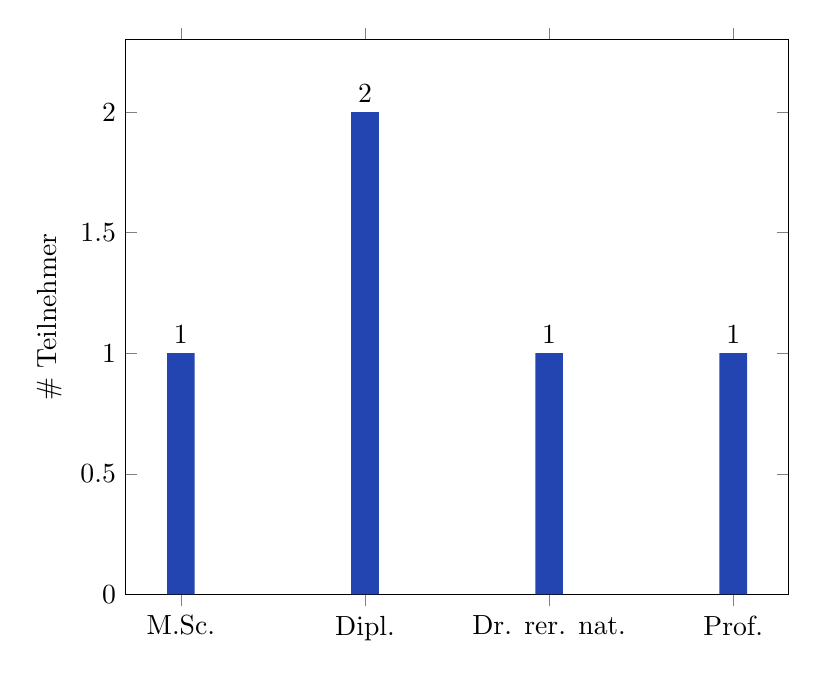
\begin{tikzpicture}
\begin{axis}[
    ybar,
    ymin=0, ymax=2,
    enlarge y limits={0.15,upper},
    ylabel={\# Teilnehmer},
    symbolic x coords={M.Sc.,Dipl.,Dr. rer. nat.,Prof.},
    xtick=data,
    nodes near coords,
    nodes near coords align={vertical},
    ]
\addplot [draw=none,fill=darkblue] coordinates {(M.Sc.,1) (Dipl.,2) (Dr. rer. nat.,1) (Prof.,1)};
\end{axis}
\end{tikzpicture}
\end{frame}

\begin{frame}{Ein paar Statistiken}{Code-Komplexit\"at}
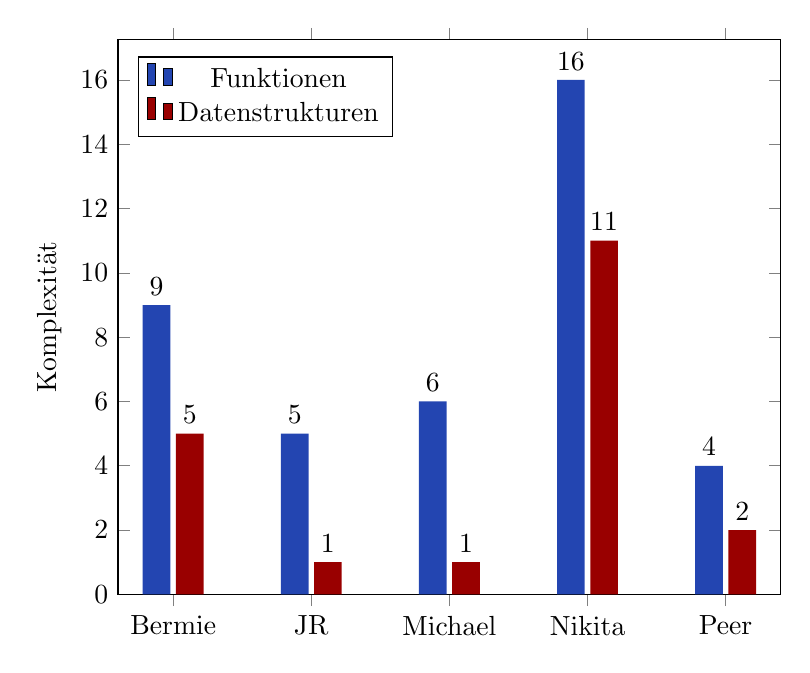
\begin{tikzpicture}
\begin{axis}[
    ybar,
    ymin=0, ymax=15,
    enlarge y limits={0.15,upper},
    ylabel={Komplexit\"at},
    symbolic x coords={Bermie, JR, Michael, Nikita, Peer},
    xtick=data,
    nodes near coords,
    nodes near coords align={vertical},
    legend pos=north west
    ]
\addplot [draw=none,fill=darkblue] coordinates {(Bermie,9) (JR,5)
  (Michael,6) (Nikita, 16) (Peer, 4)};
\addplot [draw=none,fill=darkred] coordinates {(Bermie,5) (JR,1)
  (Michael,1) (Nikita, 11) (Peer, 2)};
\legend{Funktionen, Datenstrukturen}
\end{axis}
\end{tikzpicture}
\end{frame}

\begin{frame}
\centering
\Huge \color{darkblue} Code-Pr\"asentation
\end{frame}

\begin{frame}{Auswertung}
\begin{itemize}
\item Sortierung von Listen: Mengen als Datenstruktur besser geeignet
\item Verschiedenheitstest: Kennzeichnung einzigartiger Einheiten
\item All- und Existenzaussagen: Funktionen herausabstrahieren
\item Eigenschaftstests: Kombinatoren herausabstrahieren
\end{itemize}
\pause
Selbst ernannte Grundvoraussetzungen:
\begin{itemize}
\item hohe Wiederverwendbarkeit
\item gewisses Ma\ss{} an Nat\"urlichsprachlichkeit
\end{itemize}
\end{frame}

\begin{frame}{Auswertung}{Recherche}
\begin{tabular}{ll}
\hline
\hline
\large \textbf{Pattern} & \large\textbf{Example}\\
\hline
\emph{PNoun} is a \emph{CNoun}. & Roberta is a person.\\
\emph{PNoun} is \emph{Adjactive}.& Roberta is female.\\
A \emph{CNoun} is \emph{Adjactive}. & A person is female.\\
\emph{CardRest} \emph{CNoun} \emph{Verb} a \emph{CNoun}.
 & Every person holds a job. \\
\hline
\hline
\end{tabular}
\vfill
\footnotesize Rolf Schwitter; The jobs puzzle: Taking on the challenge via controlled natural language processing.
\end{frame}

\begin{frame}[fragile]{Auswertung}{Erste Entw\"urfe}
\begin{lstlisting}
data Gender = Male | Female
data Job = Boxer | Chef | Guard | ...
data Person = Person { gender :: Gender, job :: Job }

prop1  = (roberta `hasNot` job) Boxer
prop2a = (roberta `has` gender) Female
prop2b = roberta `is` female
\end{lstlisting}
\end{frame}
\end{document}
